\documentclass[12pt,a4paper,norsk]{article}
\usepackage[norsk]{babel}
\usepackage[utf8]{inputenc}
\usepackage{parskip}
\usepackage{graphicx}
\usepackage[top=3.0cm, bottom=2.5cm, left=3.0cm, right=3.0cm]{geometry}
%\usepackage{amsmath}
%\usepackage{amssymb}
%\usepackage[nottoc]{tocbibind}
%\usepackage{tocloft}
%\setlength\cftbeforetoctitleskip{-1cm}
%\usepackage{float}
%\usepackage{subcaption}
%\usepackage[labelfont=bf]{caption}
%\usepackage[hidelinks]{hyperref}
%\usepackage{listings}
%\usepackage[libertine]{newtxmath}
%\usepackage[no-math]{fontspec}
%\usepackage{libertine}
%\usepackage{titlesec}
%\newfontfamily\secfont{Source Sans Pro}
%\titleformat*{\section}{\Large\bfseries\secfont}
%\titleformat*{\subsection}{\large\bfseries\secfont}
%\setmonofont[Scale=0.8]{Source Code Pro}
%\lstset{basicstyle=\linespread{0.9}\ttfamily, breaklines=true, xleftmargin=.21in, showstringspaces=false}

\begin{document}
\begin{titlepage}
    \centering
    \vfill
    {\bf\Large
        TTM4100 \\
        Chat-prosjekt \\
        \vskip2cm
        Group 82
    }

   {\large
   Rubin Gerritsen\\
   Simen Haugo\\
   Erik Liland\\
   Kristian Roaldsnes\\
   Øyvind Wilson
   }
   \vfill
   \vfill
   \tableofcontents
   \vfill
\end{titlepage}

\section{Beskrivelse}
\subsection{Generelt}
Vi har valgt å implementere dette prosjektet i Go, da dette er et språk som har en god idiomatisk støtte for flere-tråd applikasjoner. Kommunikasjonen mellom trådene er basert på kanaler, som gjør deling av data mellom flere tråder enkelt og sikkert. Figur (\ref{class}) viser hovedoppdelingen av prosjektet. Figur (\ref{seq_client}) og (\ref{seq_server}) viser hvordan meldingsflyten typisk vil se ut på klient- og server-siden.

\subsection{Klient}
Klienten kommer til å bestå av tre tråder:
\begin{enumerate}
	\item (main) Kjører initialisering av kommunikasjonskanaler mellom trådene, oppretter TCP-forbindelse med serveren og starter de to andre trådene. Tar imot nettverkspakker fra serveren og håndterer disse, tar imot input fra brukeren (gjennom en kanal) og sender dette videre til serveren.
	\item (nettverkslytter) Blir startet med en opprettet TCP-socket og en kommunikasjonskanal som argumenter. Kjører loop på lesing av socketen, og returnerer ferdig dekodede pakker til ”main” gjennom en dedikert kanal.
	\item (bruker-input-lytter) Blir startet med en kanal som argument, og bruker denne kanalen til å returnere strenger som brukeren gir gjennom tastaturet.
\end{enumerate}

\subsection{Server}
Serveren kommer til å bestå av 2 tråder + 1 tråd per bruker:
\begin{enumerate}
	\item (main) Kjører initialisering av kommunikasjonskanaler og starter en ny tråd som tar seg av TCP socket og innkommende forbindelser. Etter initialiseringen tar main seg av all server-logikken:
	\begin{enumerate}
	\item For hver nye TCP-forbindelse som tråd2 får inn, starter main en ny tråd som tar seg av meldinger fra denne brukeren.
	\item For hver melding som kommer fra en bruker, returneres respons etter spesifikasjonen.
	\end{enumerate}
	\item (TCP-lytter) Oppretter en TCP-socket som tråden lytter på. Kjører loop: Når en ny klient ønsker å koble seg på, aksepteres denne tilkoblingen og den nye socketen blir sendt til main for videre håndtering.
	\item (Bruker-tråd) Opprettes en tråd per bruker som leser socketen til denne brukeren, og returnerer en dekodet pakke til main når den får inn meldinger.
\end{enumerate}
\newpage

\section{Klassediagram}
\begin{figure}[ht!]
    \centering
    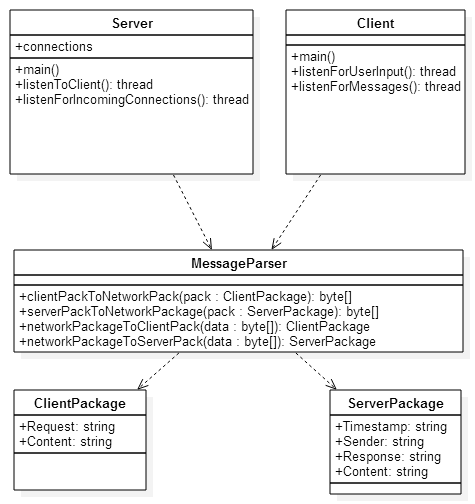
\includegraphics[width=\textwidth]{class_diagram.png}
    \caption{Hovedoppdeling av prosjekt}
    \label{class}
\end{figure}
\newpage

\section{Sekvensdiagram}
\begin{figure}[ht!]
    \centering
    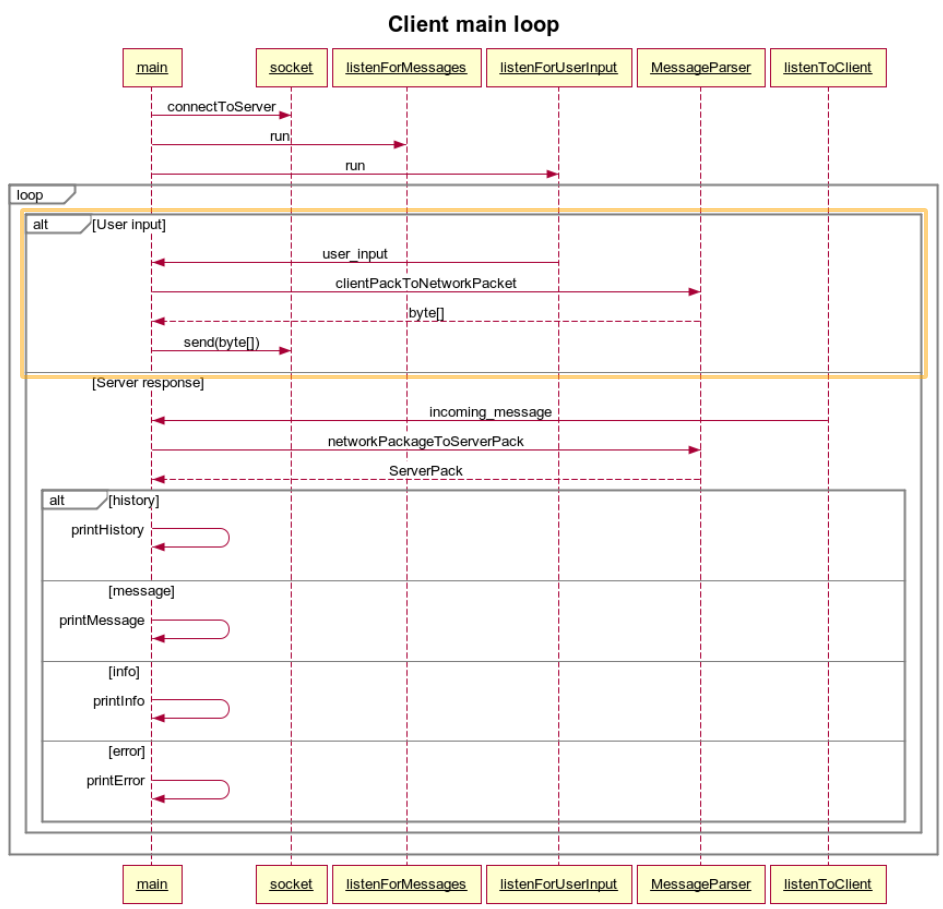
\includegraphics[width=\textwidth]{sequence_client_main.png}
    \caption{Sekvensdiagram for klient}
    \label{seq_client}
\end{figure}

\begin{figure}[ht!]
    \centering
    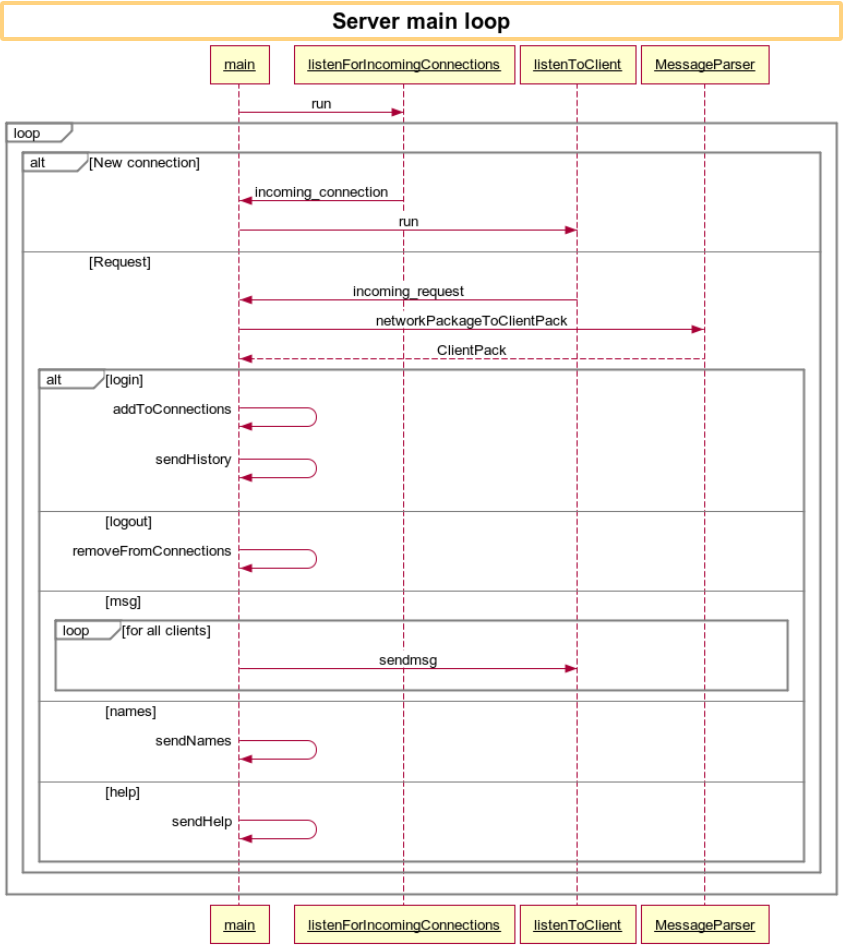
\includegraphics[width=\textwidth]{sequence_server_main.png}
    \caption{Sekvensdiagram for server}
    \label{seq_server}
\end{figure}

\end{document}
